% Here is a suggested template for PhD research proposal for the
% first annual report.
% Written originally 2010-06-22 by T. W. Yee.
% Last modified      2010-07-22 by T. W. Yee.


\documentclass[12pt,a4paper]{article}


 \usepackage{natbib}    % For BibTeX
 \usepackage{graphicx}  % To import .pdf files
 \usepackage{booktabs}
 \usepackage{comment}
%\usepackage{times}
 \usepackage{setspace}
 \onehalfspacing

 \oddsidemargin  -10mm
 \evensidemargin -10mm
 \headheight 0mm
 \headsep -3mm
\textheight 250mm
\textwidth 180mm
\topmargin -4mm
\topskip -10mm

%\textwidth=450pt
%\hoffset=-2cm

\usepackage{amsmath}
\usepackage{amsfonts}
\newcommand{\bu}{\boldsymbol{u}}
\newcommand{\bx}{\boldsymbol{x}}
\newcommand{\by}{\boldsymbol{y}}
\newcommand{\bz}{\boldsymbol{z}}
\newcommand{\bY}{\mathbf{Y}}
\newcommand{\bX}{\mathbf{X}}
\newcommand{\bZ}{\mathbf{Z}}
\newcommand{\btheta}{\boldsymbol{\theta}}
\newcommand{\mat}[1]{\mathbf{#1}}

\usepackage[acronym]{glossaries}
\newacronym[shortplural={ATIS}]{atis}{ATIS}{advanced traveller information system}
\newacronym{avl}{AVL}{automatic vehicle location}
\newacronym{gps}{GPS}{Global Positioning System}
\newacronym{api}{API}{application programming interface}
\newacronym{gtfs}{GTFS}{general transit feed specification}
\newacronym{knn}{KNN}{$k$-nearest neighbour}
\newacronym{ann}{ANN}{artificual neural networks}
\newacronym{svm}{SVM}{support vector machines}
\newacronym{kf}{KF}{Kalman Filter}
\newacronym{pf}{PF}{Particle Filter}
\newacronym{mcmc}{MCMC}{Markov chain Monte Carlo}


\usepackage[hidelinks]{hyperref}
\usepackage{cleveref}


\begin{document}

\begin{Large}
\begin{center}
\textbf{Predicting Future Arrival Times of Buses} \\
\textbf{by Tom Elliott} \\
\textbf{for a PhD in Statistics}
\end{center}
\end{Large}


\hfill{Student ID: 1596870}

\hfill{Email: tom.elliott@auckland.ac.nz}

Supervisor: Professor~T.~Lumley

% Co-supervisor: Dr~B.~Brewer

% Advisory Committee: Drs~B.~Efron, D.~R.~Cox, K.~Pearson.\footnote{
% Specify the affiliation if outside the UoA Statistics
% Department.}



\begin{center}
\today
\end{center}


This document represents the student's research proposal after
one year of provisional PhD registration.
Confirmed PhD registration is now sought.




% ----------------------------------------------------------------------
\section{Introduction}
\label{sec:intro}



% This document is a template that can be edited by the student.
% Fill in the details as you go along and delete these instructions.
% Do have your research proposal scrutinized by your supervisor before
% submitting it to the department.



% Give a few paragraphs here on the general background
% to your research proposal; put the full details in
% Section~\ref{sec:background}. You might want to cite a few
% previous important results/papers. Describe any theory briefly
% here but put most of the details in Section~\ref{sec:background}.
% Describe any data in general with a few lines here but put the
% full details in Section~\ref{sec:data}.


% Motivate this section well \ldots why is the topic important?
% What use will the thesis have?
% What is unknown that will be known upon completion?


% This section should be understandable by an intelligent person
% who is not familiar with the technical details involved.
% The reader should be convinced that your work
% is worthwhile.





% Some of our PhD students have published in the primary literature
% directly using material from their thesis,
% e.g.,
% \cite{wors:1979},
% \cite{yee:wild:1996},
% \cite{wild:yee:1996},
% \cite{murr:1999},
% \cite{jian:scot:wild:2006},
% \cite{roev:meye:etal:2007},
% \cite{mill:stew:2007},
% or submitted such as
% \cite{lee:hiro:2008}.
% Ideally you should aim at least one of your publications towards
% a mainstream statistics journal, preferably your first one.
% All publications should be in a peer-reviewed international journal.
% It should be in the primary literature.
% Statistical theory and methodology is to be regarded as the highest
% form of quality output.
% Accompanying high quality software that can easily be used
% by others (such as a R package) is also good.
% It is best to submit to journals before the completion of a thesis
% because an acceptance validates the quality of that research.



% A word about writing up your thesis.
% In general, the Department of Statistics recommends \LaTeX{} rather than
% Microsoft Word.
% \LaTeX{} is easily run on the Department's Linux machines.
% A website that converts pdf into Word is \textsf{www.pdftoword.com}.
% The University of Auckland offers a half-day workshop
% on \LaTeX{} to postgraduate students.
% There is Sweave \citep{lmucs-papers:Leisch:2003b} which allows R
% \citep{R:Ihaka+Gentleman:1996} to be embedded into a \LaTeX{}
% document, and so the output does not have to be manually
% cut-and-pasted in. Sweave is useful for presentations too,
% in conjunction with Beamer.


% There is an editor called Emacs which is useful for all types of
% editing, including \LaTeX{}, C, and R.
% In Windows there is Tinn-R for R files and MiKTeX for \LaTeX{}.


% Note that {BibTeX} items are available from MathSciNet
% which is part of the ``Library Databases'' in the UoA electronic library
% system.
% There is a close relationship between EndNote and {BibTeX}.

\textbf{Background:}
Public transport is central to city planning and traffic management in large cities.
There are various forms, including trains, trams, ferries, and of particular interest to us, buses.
Over the years, the technologies involved in these systems has become ever more complex,
one evident example being the introduction of cashless payment systems such as 
Auckland Transport's HOP cards \citep{cn}.

Another technology that is widely used in public transport vehicles is positioning devices,
referred to in the literature as automatic vehicle location (AVL) systems.
Once such system is the global positioning system (GPS),
which is used by many transit providers, including Auckland Transport.

\textbf{The main purpose:}
As a result of this real-time location information, many studies have investigated methods of
predicting travel time of buses (and hence arrival time at future stops).
The goal of these studies was to make accurate predictions about the estimated time until arrival (ETA) 
of a bus for passengers waiting at a bus stop.
Consequently, studies have shown that when a countdown is displayed, percieved waiting times are less 
than actual wait times \citep{cn}.
However, this is only true so long as the countdown is accurate.

In Auckland, there are two main cases where inaccuracy can cause frustration for passengers:
the first is when uncertainty is large, and ETAs can increase suddenly, 
while the second occurs when a bus that is not running for whatever reason is still displayed 
on the board, so commuters are left waiting for a bus that isn't coming.
The first of these is an issue we will be targeting, while the second may only be something we can allow for.


\textbf{Work that has been done:}
Previous studies have used a range of different modeling and prediction techniques to obtain ETAs.
These ranged from fairly simple real-time only Kalman Filter models \citep{cn}, 
to data-driven models such as 
$k$-nearest neighbour (KNN) \citep{cn}, 
artificial neural networks (ANNs) \citep{cn}, 
and support vector machines (SVMs) \citep{cn}.
Recently, several particle filter models have been used in various ways to solve transit problems,
such as \cite{hans-etal:2015} who used a particle filter to model the bunching behaviour of buses
in the hopes of coming up with better management techniques.



\textbf{What we hope to achieve:}
There are several areas we hope to target in our research.
The first of these is to improve predictions by using more of the available data,
including travel times of other buses traveling along the same road ways, 
not necessarily the same route.
The second is to investigate predictions intervals as a way of communicating uncertainty to commuters.
Finally, we hope to create a user interface (UI) that allows commuters to (i) find out the ETA of their bus,
and (ii) a journey planning application that lets commuters choose the best (fastest) journey to their destination.

To do all this, we are going to focus on implementing a particle filter to model the dynamic motion of buses,
and use this in conjunction with historical data and the travel times of other buses to estimate ETA.



% ----------------------------------------------------------------------
\section{Background}
\label{sec:background}


% Background knowledge is crucial, therefore describe it fully here.
% Specify the background to the problems you are trying to solve.
% Define anything technical that most statisticians will not be
% familiar with.


% What previous work has been done in the area?
% Cite references relating to such work, e.g.,
% in the form of \cite{reid:2003} and \cite{efro:tibs:1993}.
% Has anybody described any open problems in the literature?


% Make sure that problems arising from the background knowledge
% are clearly described. There should be a logical flow of thought
% in this section starting from the background and leading to the
% problem on hand.




% Don't put anything new in this section.


Since as early as 1995, public transit agencies have been deploying \gls{avl} systems
in their fleets.
The purposes of these systems range from operational, such as planning and maintenance, 
to \glspl{atis}, most notably real-time arrival information and journey planning
\citep{tcrp:2003}.
One of the more common types of \gls{avl} is the \gls{gps},
which is what our work will focus on.


In a \gls{gps}-based \gls{avl} system, vehicles report their position to dispatch
at regular intervals, approximately every 30~seconds,
which can then be accessed through public \glspl{api} if it is provided by the agency
\citep{tcrp:2003}.
The particular family of \gls{api} we will be working with is \gls{gtfs}
(see section~\ref{sec:data}).



\subsection{A History of Bus Arrival Prediction}
\label{sec:history}


The simplest arrival time prediction techniques use a combination of arrival times at previous stops
and travel time between stops.
In this, the arrival time of the current bus at its last stop is recorded, 
and then travel time between the last stop and the next one, provided by previous buses,
is added to it to predict arrival time at the next stop.

An alternative algorithm was implemented by \cite{dailey:2001} in Seattle, Washington,
in which a Kalman Filter approach was used to predict arrival time in a situation where
actual arrival time at previous stops was unknown.
The system used signpost and an odometer to determine the location of a bus and its 
distance into a trip rather than \gls{gps} location.
\cite{cathey-dailey:2003} produced a general prescription for arrival time prediction using
\gls{avl} data, including \gls{gps}.
In this, they described a three part algorithm:
the first part involved the ``tracker'', in which GPS location was converted to distance into trip
based on static schedule information;
the second involved estimating the \emph{true state} of the vehicle (distance into trip, speed, 
and acceleration) using a Kalman Filter;
and the third part presented predictors that could use the estimated state to generate arrival time predictions.


Over the next decade, many other prediction algorithms were proposed, compared, and implemented.
These included several data-driven models such as \gls{knn} regression,
\gls{ann}, and \gls{svm} 
\citep{chang-etal:2010,jeong-rilett:2005,yu-etal:2006,yu-etal:2010,yu-etal:2011}.
In these, historical data is collected over a period of time,
and then real-time data is used to obtain arrival time predictions, 
based on what was observed historically.


A more recent approach to modeling the state of transit vehicles is the particle filter,
which has been shown in many transportation studies to outperform the Kalman Filter
\citep{chen-rakha:2014,cn}.
In their work, \cite{chen-rakha:2014} used a particle filter to predict travel times,
while \cite{hans-etal:2015} used a particle filter in an operations research and control setting,
in which their goal was to propose control strategies to reduce the bunching of consecutive buses
along a common route.
As far as we can tell, the particle filter has not been used as a predictive model for
arrival times, nor has it been applied to a general GPS-based system in which actual arrival times
are unknown.




\subsection{Recursive Bayesian Filters}
\label{sec:recursive}


Of the many approaches to modeling real-time bus positions discussed in \cref{sec:history},
our work will be focussing on recursive Bayesian filters.
These are a class of model specially suited to data that is observed over time,
and in most cases analysed in real-time.
In our case, the observations are of bus locations,
which we wish to analyse use to make future arrival time predictions in real-time.


In the general framework of recursive Bayesian filters,
there is a true state $\bX_k$, which is unknown and unmeasurable.
However, there is also a \emph{hiden Markov process},
which has state $\bY_k$ that is dependend on $\bX_k$, 
for which we can make observations.


In our case, the true state is the \emph{distance into trip}, $d_k$, 
and speed, $v_k$, of a bus.
That is, $\bX_k = [d_k\ v_k]^T$.
However, we only have access to measurements of the GPS position, 
(latitude and longitude), 
as well as the time since the last observation, $\delta_k$,
so the observation state is $\bY_k = [\phi_k\ \lambda_k\ \delta_k]^T$.



\subsubsection{Kalman Filter}
\label{sec:kalman_filter}

Of the various recursive Bayesian filters, one that has been predominant in 
many real-time applications which, apart from its use in buses described here,
has also had military applications such as submarine and missile navigation, 
is the \gls{kf}.
It most of these applications, the models are fairly simple and use only
linear state transition equations (such as Newton's Laws of Motion),
and Gaussian noise is an adequate assumption \citep{cn}.


In a \gls{kf}, the model assumes that there is a known, linear state transition specified by
a matrix $\mat{A}$, with Gaussian process noise $\mat{w}_k$.
That is, 
\begin{equation}
  \label{eq:kf_statetransition}
  \bX_k = \mat{A}\bX_{k-1} + \mat{w}_k.
\end{equation}
The relationship between the unknown state and the hidden Markox state is described
by a measurement matrix $\mat{H}$, along with the measurement error $\mat{v}_k$,
\begin{equation}
  \label{eq:kf_measurement}
  \bY_k = \mat{H}\bX_{k-1} + \mat{v}_k.
\end{equation}
The limitation here is that the relationship between $\bX$ and $\bY$ needs to be a linear
combination of the state parameters.


The \gls{kf} works in two steps.
First, the new state is \emph{predicted} from the previous one, $\hat\bX_k = \mat{A}\bX_{k-1}$,
and then the state is \emph{updated} using the observations.
Each state is associated with a mean vector (the state) and associated covariance matrix.
In this way, the state is assumed to have a multivariate normal distribution.


In the \gls{kf} implementation described by \cite{cathey-dailey:2003},
they were required to first estimate the distance into trip to make observations 
$\bZ_k = \mat{H}\bX_{k-1} + \mat{v}_k$, where $\mat{H} = [1\ 0]$.
These approximated observations are then what was used to update the state.
Along with the Gaussian assumptions of all errors,
this makes the \gls{kf} somewhat restrictive,
and not ideal for modeling processes which to not obide strictly to linear dynamic equations.



\subsubsection{Particle Filter}
\label{sec:particle_filter}

In response to the restricted nature of the \gls{kf}, there have been many 
alternatives described, such as the Extended Kalman Filter,
but the one we are most interested in is the \gls{pf}.
This generalised model allows us to use unrestricted \emph{functions} to model
state transitions and measurement, rather than be limited by matrices.


Instead of modeling the state distribution, the \gls{pf} instead uses a sample of independent 
state estimates, which can each be modeled individually, and then resampled using the observed data.
Similar to a standard \gls{mcmc}, the sample can be used to make inferences about the true state.
In our case, we assume to bus starts with a state of $\bX_0 = [0\ v_0]^T$,
where $v_0$ is given a useful prior distribution, 
or may be based off of the state from a previous trip.
Therefore, an individual particle is denoted $\bX_0^{(i)} = [0, v_0^{(i)}]^T$.


Once a prior distribution of particles is generated, 
we can model each one individually (and independently) using the state transition function,
as well as any other information we have available (see \cref{sec:busbehavior}) and process noise,
\begin{equation}
  \label{eq:pf_statetransition}
  \bX_k^{(i)} = f(\bX_{k-1}^{(i)}, \ldots, \mat{w}_k^{(i)}).
\end{equation}
Now, since each particle has an estimate of $d_k$, we can use the shape information to
find the GPS location of that particle,
\begin{equation}
  \label{eq:pf_measurement}
  \bZ_k^{(i)} = h(\bX_k^{(i)}).
\end{equation}
We can then use the distance between two GPS coordinates to weight the particles (the likelihood),
and use these weights to resample and generate a posterior distribution of the new state.


The main advantage of the \gls{pf} is that we make unnecessary assumptions about the distributions
involved, and we are not restricted to linear transitions between states (except for computational
complexity).
One of the key features here, which is unique to modeling buses, 
is \emph{dwell times}, which are discussed in \cref{sec:busbehavior}.
In a \gls{kf} framework, it is very difficult, or perhaps impossible, to accurately
model dwell times;
with a \gls{pf}, however, we only need to worry about each particle.
Given a sample of particles, we can allow each one to stop with some prior probability,
so that we end up with a multi-modal distribution of particles; those that stopped, 
and those that didn't.








% In a traditional modeling framework, all of the observations, $\bY$, are available before
% the analysis begins.
% In this case, the posterior distribution of the parameters, $\btheta$, is
% \begin{equation}
%   \label{eq:bayes_theorem}
%   \pi(\btheta|\bX) \propto \ell(\bX | \btheta) \pi(\btheta)
% \end{equation}
% where $\ell$ is the likelihood function of the data.

% When dealing with real-time observations, however, it makes more sense to update
% the posterior with the latest observation.
% This framework is known as recursive (Bayesian) filtering.
% A well known example is the \gls{kf},
% which has been used in bus arrival prediction since the 1990's \citep{cn}.

% The basic set up of the \gls{kf} is to start with a prior distribution,
% $\bX_0$, that represents some unknown \emph{state} of the system.
% For example, $\bX$ may be a vector of a vehicle's position and speed.
% Every time a new observation is recorded, the previous state is first used
% to \emph{predict} what the new state will be, 
% and then the observation is used to \emph{update} this state,
% allowing for measurement error.

% The main restriction of the basic \gls{kf} is that the model assumes the state $\bX$ 
% is multivariate normal, and the algorithms work directly with the mean (vector)
% and covariance matrix.
% In this way, the \gls{kf} can be very fast, especially when $\bX$ has only a few
% parameters.


% Some examples of \gls{kf} in buses \ldots



% Originally called a ``bootstrap filter'', the particle filter (PF) was first proposed by
% \cite{gordon-etal:1993} as a recursive Bayesian filter that needn't impose unnecessary assumptions,
% such as linearity and Gaussian noise in a Kalman Filter (KF).
% In their simulation example, the PF greatly outperformed the KF,
% a result which has been restated in successive studies
% including one by \cite{gustafsson-etal:2002} whose work involved position, navigation, and tracking.


% Similar to the KF, the PF involves two main steps.
% First, proposals are made which form the prediction step.
% Unlike in a KF, however, these proposals have no restrictions, and so can be any
% desired function;
% predictions are made for each individual particle, rather than the estimated state as a whole.
% Second, the particles are resampled, with replacement, using weights determined by the likelihood
% of each particle given the latest observation.
% The main advantage of using the PF is that no unnecessary assumptions need to be made. 


% Let us denote the (current) state by $x_k$, which we want to corresepond in some way to the as yet
% unavailable observation $y_k$.
% In general, we will define a function $h$ mapping the state to the observation,
% such that $h(x_k) = y_k$.
% Before observing $y_k$, we need to estimate $x_k$ based on $x_{k-1}$ and any other information
% we have available (such as schedule information or historical data),
% as well as process noice, $u_k \sim \mathcal{N}(0,\sigma^2)$\footnote{this doesn't necessarily need to be Gaussian}.
% That is, $\hat x_k = f(x_{k-1}, \mathbf{D}) + u_k$.

% In the context of particle filtering, the function $f$ is unrestricted (except by computational complexity).
% Therefore, $f$ can describe the behaviour of an individual \emph{particle}, $x_{k-1}^{(i)}$, 
% rather than the entire distribution of $x_{k-1}$.
% This is especially useful in the context of bus behaviour as multimodality is common,
% for example a bus can either stop and wait at a bus stop, or it can drive past without stopping
% (see section~\ref{sec:busbehavior}).
% Thus, the prior state estimate $\hat x_k$ is represented 
% by a sample of particles $x_k^{(i)} = f(x_{k-1}^{(i)}, \mathbf{D}) + u_k^{(i)}$.


% Once the data is obtained, Bayesian bootstrapping is used to resample the prior samples to generate
% a posterior distribution for $x_k$.
% This is achieved using the likelihood, $\ell(y_k | h(\hat x_k), \sigma_y^2)$,
% where $\sigma_y^2$ represents the measurment (i.e., GPS) error,
% to obtain sampling weights for each particle:
% \begin{equation}
%   \label{eq:particle_weights}
%   w_i = \frac{\ell(y_k | h( x_k^{(i)}), \sigma_y^2)}{\sum_{j=1}^M \ell(y_k | h( x_k^{(j)}), \sigma_y^2)}
% \end{equation}

% Again, $\ell$ is unrestricted in a PF framework, however in our situation it makes sense to 
% compute the (Great Circle\footnote{this automatically accounts for differences in the scale of latitute
% and longitude}) 
% distance between each particle and the true position:
% closer particles will have higher weights than those farther away.
% The new sample is then used to predict the future state $x_{k+1}$.







\subsection{Modeling Bus Behavior}
\label{sec:busbehavior}


One unique feature of model bus behaviour is that they can stop and wait at bus stops along the route
while passengers get on and off.
The time spent waiting at a stop is known as \emph{dwell time},
and has been shown to be necessary in accurately modeling bus behavior \citep{cn}.
Algorithms such as the KF cannot easily incorporate dwell times,
as they need to occur with some probability (the bus doesn't \emph{have} to stop).
The PF, however, has no such difficulty,
and \cite{hans-etal:2015} describe how they applied a PF to buses.


When approaching as bus stop,
each particle can independently decide whether or not it will stop,
and depending on the outcome follow the relevant trajectory.
Those particles that do stop will each be given (independently)
a dwell time, after which period they will continue along the route.

Inevitably, when passing a stop, the prior distribution of the particles will be multimodal:
those that stopped, and those that didn't.
In their work, \cite{hans-etal:2015} also had data relating the traffic light locations and
timings, so they were able to do a similar model in that regard.
However, Auckland Transport currently has no such data publicy accessible,
so we are unable to implement their models.



\subsection{Predicting Arrival Time}
\label{sec:arrivaltimeprediction}

Arrival time prediction has been evolving since some of the first \gls{avl}
systems were installed in bus fleets.
Prediction methods range from simple carry-on delay,
do much more complicated prediction functions involving historical data,
dwell time distributions, 
and headway (the time between the last bus to travel the route and the current one).


Delay models \ldots
\cite{dailey:2001} just used state, arrival time, and delay.


\cite{cathey-dailey:2003} included several examples of arrival time prediction models
that could incorporate historical data, etc.
KF to estimate state, then use that state to predict arrival time.


Others, using KNN, ANN, SVM etc. use historical data to combine current
realtime location to predict arrival.
Including use of routes with multiple buses, recent travel times, etc.


Other more advanced methods, \cite{hans-etal:2015} use PF to predict arrival.
Other PF models that use historical data as particle trajectories.


Doesn't look like there have been any uses of big-data models that use
historical data of \emph{all} buses traveling along a road
(not just those of the same route) as well as the same real-time data,
and then making predictions using all of this.







% \textbf{What are we trying to do? }
% Prediction of travel (or arrival) time has many applications,
% for instance optimising traffic flow, priortising traffic signals,
% and improving the behaviour of vehicles on multiple-vehicle routes
% \citep{hans-etal:2015}.
% The application we are interested in, however, is providing commuters with accurate predictions of 
% the question every bus-commuters asks, ``how long will I be waiting here?''.


% \textbf{Why are we trying to do it?}
% There is always going to be room for improvement when it comes to predictions.
% However, it seems that the predictions in Auckland are often wrong,
% and it is of particular interest to us to come up with better predictions.



% \textbf{How are we going to make predictions?}
% Making predictions about travel or arrival times (knowing the travel time between two points
% tells you the arrival time at the later point) consists of two parts:
% the first involves accurately modeling the dynamic state of the vehicle
% (that is, its current position, refered to often as ``distance into trip'', its speed,
% and its acceleration).
% The second step uses the dynamic state to predict the path of the vehicle,
% and thereby estimate the travel time to and arrival time at a point in the future (i.e., a bus stop).

% These two can be treated using a single model \citep{cn},
% or as two related but separates models \citep{cn}.
% The latter is what we will be using, as it is more flexible and allows the incorporation of more information.
% For the first part, we will use a particle filter based on
% (i) the state-space of the vehicle (distance into trip, velocity, and acceleration),
% or (ii) historical data for the given vehicle or route,
% or (iii) historical data from the most recent vehicle traveling along the given route,
% or (iv) a combination of (i)--(iii).

% The second part (prediction) will involve similar information, and is where most of the work will be done.
% In fact, the only difference between the two is that the first predicts the distance into trip after a given
% length of time, while the second predicts the time taken to travel a given distance.
% The first is over short time periods (10-60~seconds), 
% while the second could be making predictions up to an hour in advance, so there is a lot more room for variability.

% The final part of the project involves communication of this information to commuters.


% \textbf{What's already out there?}
% Kalman Filter, KNN, ANN, SVN, and many others \ldots including particle filters (only recent, 2014).

% \textbf{What can we do better?}
% Use more relevant data (congestion, historical, etc).
% Make more useful predictions (different point estimate, prediction intervals, \ldots).
% Better models that don't have fewer assumptions and overcome some problems 
% (e.g., particle filter that doesn't make assumptions about distributions, etc).


% Predicting the arrival time of a bus at a future stop is done in two stages:
% a \emph{modeling phase}, and a \emph{prediction phase}.
% The modeling phase uses the real time location data to estimate a dynamic system.
% That is, the \emph{true} location and velocity of the vehicle in question,
% accounting for measurement error.
% The prediction phase uses the information from the model, and any other sources of useful information,
% to forecast the state of the system and make predictions about the arrival time at future locations (i.e., stops).


% There are several ways to model the system, the most common of these being the \emph{Kalman Filter}.



% \subsection{Modeling AVL Data}

% To model transit vehicle location, we use a state-space model.
% This is dynamic in position, velocity, and acceleration.
% Early models map the reported location of a vehicle from two dimensions into one,
% by estimating the ``distance into trip''.
% This distance can then be modeled using various techniques, 
% and use the state of the vehicle at the previous time point to predict and update the model.
% The Kalman Filter is the most popular example of this, and is useful for real time applications
% because it is fast: only a single iteration is required for each new observation, and requires only matrix manipulation
% \citep{cathey-dailey:2003,cn}.
% The details of the KF are given in \S\ref{sec:kalman_filter}.


% Other methods of modeling have been used and compared over the last decade.
% These include regression models \citep{cn}, 
% K-nearest-neighbour \citep{cn}, 
% artificial neural networks (ANNs) \citep{cn},
% scaled vector machines (SVMs) \citep{cn}, 
% and others.


% An extension of the KF that hasn't been used in transit predictions is the particle filter (PF),
% likely due to the computational requirements of the model.
% However, we believe it may be a viable alternative that will provide a more flexible model that
% makes fewer assumptions (such as normality).
% The workings of the PF are detailed in \S\ref{sec:particle_filter}.


% \subsubsection{Kalman Filter}
% \label{sec:kalman_filter}

% The KF is at its root a recursive application of Bayes' rule.
% The idea is that, instead of fitting the model to the full set of data,
% the model is fit using one observation at a time.
% This is obviously advantageous when it comes to modeling real time data,
% as we want to \emph{update} the current sate (which contains the information from all previous observations)
% when new data is obtained,
% rather than estimate a new posterior using all of the data each time, which is (more) computationally intensive.

% Given a state vector $\bx_k = \left[d_k, v_k, a_k\right]^T$, there $d_k$ is the distance into trip,
% $v_k$ is the velocity, and $a_k$ is the acceleration at time $t_k$ (observation $k$),
% $\mathbf{A}$ is the state transition matrix,
% $\bu_k$ is the control vector at time $t_k$ (i.e., any additional information),
% $\mathbf{B}$ is the control matrix (i.e., how to use the control vector), 
% and $\mathbf{G}_k$ is the random error associated with observation $k$.
% Once data $y_k$ is obtained, the difference between the estimate and the observation is $\bz_k$,
% if $\mathbf{H}$ is the measurement matrix, then:

% \begin{equation}
%   \label{eq:kalman_filter}
%   \begin{array}{r@{~=~}l}
%     \hat \bx_k & \mathbf{A}\bx_{k-1} + \mathbf{B}\bu_k + \mathbf{G}_k \\
%     \bz_k & \hat\bx_k - \mathbf{H}\by_k
%   \end{array}
% \end{equation}

% The filter works in two stages: first, predict where the state will be at time $k$, given the previous information.
% Then, update the predictions using the newest observation, account for measurement error.
% Everything is (multivariate) normal, which can be specified as a mean and (co)varaince.
% Thus, everythign simmers down to a few matrix equations:

% \subsubsection{Particle Filter}
% \label{sec:particle_filter}

% The PF is related to the KF, but rather than working with a distribution, it works with \emph{particles}.
% Each particle represents a plausible parameter value, and when new data is obtained the predicted positions of the
% particles is compared to the observation, and a new sample of particles is taken based on the likelihood of the current set of particles.
% It's like a bootstrap at each iteration, where the particles are sampled (with replacement) to generate a new sample that represents the posterior distribution.

% Use in bus prediction \ldots \cite{chen-rakha:2014,hans-etal:2015}

% Theory ... \cite{gordon-etal:1993,carpenter-etal:1999,gustafsson-etal:2002}

% Advantages ...

% Disadvantages ...

% How will it help us? ...


% \subsubsection{Historical Data}
% \label{sec:historical_data}

% Many approaches (KNN, ANN, etc) use historical data to make predictions.


% \subsection{Predicting Arrival/Travel Times}
% \label{sec:predicting_arival_times}

% Modeling the dynamic state of the vehicle is only the first part of the problem.
% Next, this state needs to be projected into the future to make predictions about
% the arrival times at points in the future.

% In the KF implemented by \cite{cathey-dailey:2003}, 
% a prediction model is used that takes the dynamic state information and predicts the arrival times.
% Other methods use historical information to compare the current state with those observed before,
% and use that to predict arrival times.

% We want to investigate first using the PF's particles, and project each of them into the future, 
% and use that to infer predictions.

% There are also some specific problems we hope to address:

% - changes in ETA

% - missing buses

% - using data from other buses to improve predictions along a stretch of road/route 


% \subsection{Providing the Information to Commuters}
% \label{sec:information_to_commuters}

% Getting the information to commuters is also important.
% We have arrival time estimates along with the variabiltiy associated with them.
% We need to let commuters know how long they \emph{might} be waiting in best \emph{and} worst case scenarios.

% Web apps were used by \cite{cathey-dailey:2003}, and there are also phone apps to download.
% AT has a ``Where's My Bus?'' app that shows the GPS location of the bus you are waiting for.

% Journey planning, allowing commuters so provide a location and destination, 
% and get information about the best stop to walk to and bus to catch.

% Prediction intervals \ldots \cite{mazloumi-etal:2011}


% \vspace{1cm}
% \hrule
% \vspace{1cm}


% Accurate prediction of bus arrival (or departure) time from bus stops is dependent on many components.
% The primary component is the AVL system used to track the real-time positions of vehicles.
% A statistical model is then applied that uses this AVL data to model the movement of the bus over time. 
% Using this model, predictions of arrival/departure time can be made.


% There are many forms of AVL, although the most common (and the one we will be working with) is GPS.
% In this, each AVL report contains the time, vehicle information (identification, possibly trip and/or ``block'' ID,
% and the GPS coordinates).

% Google has standardised the AVL system into GTFS\footnote{\url{https://developers.google.com/transit/gtfs/}}, 
% which means any applications should be transferrable to any 
% public transport system using GTFS (Auckland Transport does, along with $M$ other companies worldwide).
% GTFS has two components: \emph{realtime} (live positioning information) and \emph{static} (schedule information,
% route shapes, timetables, etc).


% With an accessible\footnote{so long as AT makes the data available} data format, the main focus will be on algorithms
% used to model and predict arrival times. The Kalman Filter is one commonly used method for this, and has been used
% in many applications such as \cite{cathey-dailey:2003}, \cite{cn}, and \cite{cn}.
% The main idea behind this algorithm is that it is \emph{fast}: it only involves matrix operations and works with 
% the mean and variance of a normal distribution.
% No complex integrations of MCMC sampling is required.


% The KF algorithm works as follows \ldots

% Other modelling methods have been used, such as
% nearest neighbour regression \citep{chang-etal:2010},
% artificial neural network (AVN) \citep{jeong-rilett:2005}, and
% support vector machines (SVN) \citep{yu-etal:2006,yu-etal:2010,yu-etal:2011}.

% While the KF algorithm is fast and easy to use, it is limited in its assumption of normality. 
% There are multiple extensions of the KF, including the Extended Kalman Filter for using general functions, 
% and Particle Filters, which are far more flexible but require significantly more computational power.

% Particle Filtering, in the simplest of terms, requires a set of ``imaginary'' points---let's call them imaginary busses.
% Each of these is manipulated using the likelihood information to complete the \emph{prediction} step,
% which is easy enough.
% After prediction, the data is obtained and the likelihood of each virtual bus is computed,
% and a new sample is taken (with replacement) with sampling probability proportional to likelihood.
% That is, the imaginary busses closes to the real bus are sampled more often, 
% and those far away are samples less (or not at all).

% The PF can get very computationlly demanding, but it has one great advantage:
% the KF filter requires the reported GPS location to be mapped to the trip shape;
% the PF does not.
% The PF can compare imaginary GPS locations to the true GPS location, and use a bivariate normal distribution
% to estimate the likelihood (GPS's have an associated error, so we can use this or estimate it from the data).












% ----------------------------------------------------------------------
\section{So What's New?}
\label{sec:whatsnew}



% List \textit{specific} and \textit{new} results that your thesis
% plans to obtain, especially with regard to new statistical theory
% and methodology.
% It is essential that you have provided comprehensive background
% (in Section~\ref{sec:background})
% so that it is clear what new contributions will be made (here),
% and how they will extend what is currently known.
% Tie these with Appendix~A(i), and a list such as below is a
% good idea.


% For example, all of the points below are new (to my knowledge)
% and have not been done yet.
% \begin{enumerate}

% \item
% Develop a new method for quantile regression based on the
% asymmetric Laplace distribution and the concept of link functions
% and parallelism assumptions (via constraint matrices).


% \item
% Derive the asymptotic properties of the above method,
% both as $n \rightarrow \infty$ and as $p \rightarrow \infty$.




% \item
% Conduct a small simulation to check the mean squared error and
% other properties. To be done in R with some sections written in~C
% calling LINPACK \citep{dong:bunc:mole:stew:1979} for additional speed.



% \item
% Compare my results to those of~\cite{wei:carr:2009}, especially
% relating to boundary effects and small-sample properties.



% \item
% Tackle an important dataset or problem that no one has
% satisfactorily resolved before. It is essential that new
% methodologies are investigated and that novel insights are
% obtained. Note that a conventional analysis, even of a very large
% dataset, is \textit{not} PhD-level research.


% \end{enumerate}



This work will focus on three main parts:
real-time bus modeling using a particle filter,
arrival time prediction using a combination of the particle filter,
historical data, and ``real-time'' travel time information
from other buses,
and finally methods of providing this information to commuters,
including prediction intervals.


\subsection{Particle Filtering}
\label{sec:new-pf}

Unlike several other studies, including those by \cite{hans-etal:2015},
we will be working with only GTFS (realtime) data provided by Auckland Transport.
One big difference between this data and many others is that we do not have
access to actual arrival times.
For example, in the models used by \cite{hans-etal:2015},
actual arrival times were available, so they were able to use these to 
good effect in their predictions.


Instead, we will need to rely on the distribution of particles providing us
with estimated arrival times.
Each particle's arrival time can be computed, so for each stop we can obtain 
a posterior distribution of arrival times.
In most cases, this should be fairly narrow;
however, there will be situations where the bus could be traveling slow and arrive
late and have a short (or non-existent) dwell time,
or the bus could be traveling fast, arrive earlier,
and have a long dwell time.
This paragraph sucks.







\subsection{Prediction}
\label{sec:new-prediction}


Predicting bus arrival is the main goal of this work.
As we will already have a posterior distribution for the current state of
each bus, 
we will be able to use this---along with any other information we
have available---to predict arrival time.


We will be comparing various methods of prediction:
simple state prediction (that is, using only the current state of the 
bus to predict arrival time),
historical based prediction,
real-time traffic conditions obtained from other buses,
and combinations of these.
In each of these, we will allow for stopping (with probability) at stops
along the way, and the associated dwell times.




\subsection{Commuter Information}
\label{sec:commuter-info}


The end goal of our work will be a free web application available to
commuters, allowing them to check the status of their bus,
and get information regarding the estimated time of arrival.
We will investigate point estimates, as well as interval estimates to do this.


Additionally, providing ETA to destination will also be useful,
and this will pave the way for journey planning.
This is where users can enter a start and end location,
and be shown various routes they can take,
with estimates of travel time and arrival time,
allowing them to make informed decisions as to which route will get them
to their destination on time, and/or as fast as possible.





% \begin{enumerate}
% \item 
%   We're going to implement a Particle Filter to model the busses,
%   and compare it to the KF (and other methods we can get working or compare with).


% \item 
%   Then we're going to investigate better summary statistics.
%   The mean is great, but only if the posterior is normal.
%   It probably wont be, so maybe the median, or mode, or something else, will be better.
%   Also, prediction \emph{intervals}! Is the bus 2--3~minutes away, or 2--10~minutes away???

% \item 
%   Then we will use as much data as possible and see if it improves predictions 
%   (like, ``realtime'' congestion data from other busses, historical data, \ldots).

% \item 
%   Then we want to apply the methods to a real data set (Auckland Transport PTS).

% \item 
%   And then make it available via the web and/or a phone app.

% \end{enumerate}







% ----------------------------------------------------------------------
\section{Data and Special Needs}
\label{sec:data}


% Almost all Statistics PhD theses should analyse at least one
% data set, even if it is a toy data set.


% State their source fully.
% If new data is important to the thesis describe what's new.
% Why is this data set important?
% What is novel about it?
% Specify any ethics or confidentiality issues.


% A plot of some of the data may be useful;
% see Figure~\ref{fig:myfig}.


% Do you have any special needs such as IT needs?
% These include hardware (supercomputing facilities),
% and expertise/technical knowledge.
% Often extra large data sets have special needs associated
% with its processing.
% How do you invisage those needs to be met?



% Funding: anything to report here?
% If your thesis work involves experiments, travel or special
% resources in order to collect data, or essential collaboration with
% experts in your field, then you should describe these requirements
% here along with how you, or your supervisor, will fund these
% requirements. Departments work on tightly planned budgets and
% generally do not have the facilities to pay for unplanned PhD
% related expenses.



% If ethics approval(s)/permissions is needed then put
% any details here.





% \begin{figure}[tt]
% \begin{center}
% %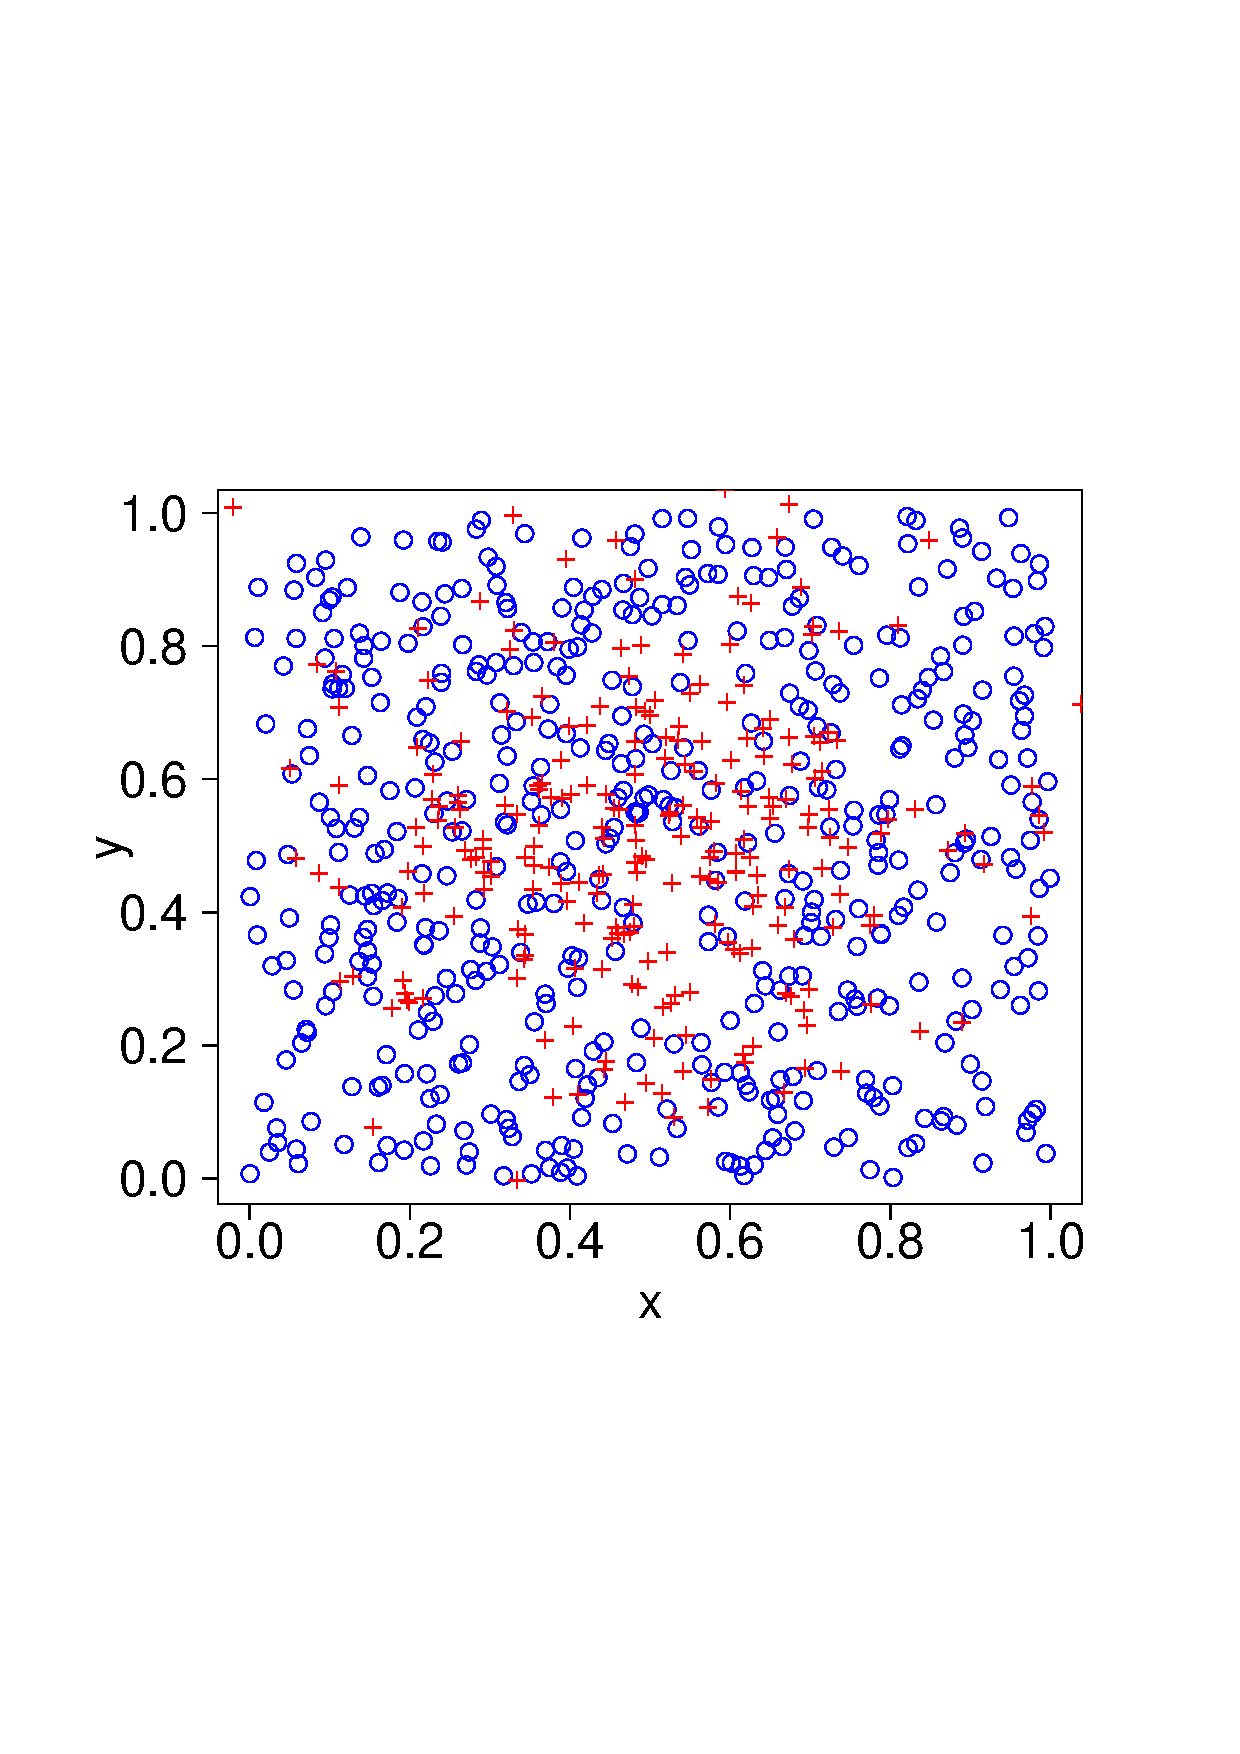
\includegraphics[height=70mm]{./myfig.pdf}
% \caption{
% Data for a two-class classification problem.
% The red ``+'' is for class~1, and $n = 250$.
% The blue ``o'' is for class~2, and $n = 500$.
% }
% \label{fig:myfig}
% \end{center}
% \end{figure}



We will need access to a GTFS realtime feed.
There a plenty of these, but we would particulary like access to Auckland Transport's.
It's on its way, apparently, otherwise we might need to sign confidentiality agreements which would be less 
fun that using open, publically accessble data.


We will eventually need a dedicated machine to run the computations continuously to provide the predictions
for the apps.
Hopefully, a low-spec machine will be enough if we can write the algorithms efficiently enough 
(a lot of the historical data can be computed at night while the busses are sleeping).
However, if more power is needed, we will cross that bridge when we get to it.
Ideally, the final ``product'' will be easy to implement on a system so can ``pass it on''
to another user (like AT) and anyone who wants it for them to maintain.





% ----------------------------------------------------------------------
\section{Goals}

% List \textit{specific} goals you wish to achieve in your PhD.


% \begin{enumerate}

% \item
% I wish to derive the first three moments of the Slash distribution.
% This will involve working out the characteristic function first.


% \begin{itemize}

% \item[a.]
% Then work out the observed information matrix
% based on~\cite{bick:etal:2009}.

% \item[b.]
% Then work out the expected information matrix
% \citep{scot:lee:wild:2007}.

% \item[c.]
% Apply the EM algorithm \citep{demp:lair:rubi:1977} to estimate~$\lambda$.

% \item[d.]
% Write a R package to implement my method.
% It will be written in S4 and use object oriented methods
% \citep{cham:1998}.

% \item[e.]
% Apply the method to the radiation data set
% \citep{MR2526777}.

% \item[f.]
% Extend biplots \citep{gowe:1966} for my data.

% \item[g.]
% Release the package on CRAN
% (cf.~\cite{murr:ihak:2000}).

% \item[h.]
% Publish my results in at least two papers,
% earmarked for JASA and JRSS-B.
% Also an applications paper in Biometrics.
% See Section~\ref{sec:timeline}.

% \end{itemize}



% \item
% Solve the Fisher-Behrens problem
% \citep{efro:2009,MR2415600,MR2508377}.


% \end{enumerate}


\begin{enumerate}
\item 
  Implement a Particle Filter on a data set and make predictions that are on par with those currently available.

\item 
  Investigate ways of using other live and historical data to improve the accuracy of estimates.

\item 
  Look at different summary statistics for better point-estimates, and look into providing useful prediction intervals.

\item 
  Implement a large-scale version of the model for a (subset of) the AT PTS, and see how well it runs.

\item 
  Create a web/phone app to access the predictions.

\item
  Package the system so that it is distributable to other feeds to remove its dependency on us.
\end{enumerate}






% ----------------------------------------------------------------------
\section{Timeline and Activities}
\label{sec:timeline}


% \begin{table}[hh]
% \caption{
% Timeline of my privisional year.
% }
% \centering
% \ ~~~~ \\
% \label{tab:timeline}
% \begin{tabular}{|c|l|}
% \hline
% Date & Activity \\
% \hline
% 2010-04-01 & Provisional PhD registration (PhD in Statistics). \\
% 2010-05-01 & Updated my personal webpage at
%              \textsf{www.stat.auckland.ac.nz/$\sim$myStudentName}. \\
% 2010-05-20 & Attended one of the
%              Doctoral Skills Programme's Induction Days. \\
% 2010-09-01 & Gave my first talk at NZSA conference. Won first prize. \\
% 2010-11-01 & Gave a talk to PhD Talks Day. \\
% 2011-01-15 & Submit my first paper to \textit{Annals of Statistics}
%              (co-authored with supervisor). \\
% 2011-05-01 & Presented my research progress to a departmental seminar. \\
% 2012-01-20 & Achieve Goal~1. \\
% 2012-08-20 & Achieve Goal~2. \\
% 2012-10-23 & Submit my second paper to \textit{Annals of Applied Statistics}
%              (co-authored with supervisor). \\
% 2013-01-15 & Submit my third paper to \textit{Biometrics}
%              (sole authorship). \\
% 2013-02-01 & Submit my PhD thesis. \\
% \hline
% \end{tabular}
% \end{table}



I have fulfulled all my first year requirements.
These are:
\begin{enumerate}

\item
All EoI provisional goals:
\begin{enumerate}

\item
\textit{Approval of the full thesis proposal by the appropriate departmental/faculty postgraduate
committee}:
Here it is!

\item
\textit{A substantial piece of written work, such as a literature review, completed to the
satisfaction of the main supervisor}: Here?


\item
\textit{Presentation of the proposal and/or work in progress to an appropriate forum e.g.\ seminar,
research group, conference, to the satisfaction of the supervisors}:
YYYY-MM-DD.

\item
\textit{Attendance at one of the Doctoral Skills Programme
Induction Days}:
2015-11-04

\item
\textit{Successful completion of the Academic Integrity Module}:
dd/mm/2014

\item
\textit{Undertake Diagnostic English Language Needs Assessment (DELNA) online screening}:
25/02/2010

\item
\textit{Complete STATS 710 and STATS 769 at B+ or higher grade within the first 
12~months\footnote{STATS 769 taught second semester, unable to complete within 12~months}
of registration}

\item
\textit{Attendance of at least 10~Statistics departmental research seminars per annum, 
with forms fully filled in and handed in}:
see Table~\ref{tab:seminars}

\item
\textit{Maintenance of a personal departmental webpage providing information on scholarly
activities and objectives to the satisfication of the supervisor and Department of Statistics
PhD Officer}:
\url{https://www.stat.auckland.ac.nz/people/tell029}

\item
\textit{Satisfactory participation in the Department of Statistics PhD Talks Day and/or give
a departmental seminar within the first 12~months of registration}:
(c)


\end{enumerate}





% \item
% I have updated my webpage
% (\textsf{www.stat.auckland.ac.nz/$\sim$myStudentName})
% giving details of my thesis, links to other research resources
% in my topic, and some personal stuff to make it interesting.


% \item
% I have diligently attend as many Statistics Department seminars
% as I could. They are given in Table~\ref{tab:seminars}.
% This is much more than the minimum quota set by the department.
% Consequently there should be no problem due to this when getting
% my annual report signed off\footnote{If insufficient seminars have
% been attended then sign off will occur \textit{after} the minimum number
% is reached.}.
% The 2010-04-08 seminar was particularly useful because it gave
% me an idea on how to solve one of my problems.


% \item
% I did STATS~730 in Semester~1 of 2010 and obtained an A+.


% \item
% I did STATS~782 in Semester~2 of 2010 and obtained an A.



\end{enumerate}











\begin{table}[hh]
\caption{
Departmental seminars I have attended.% (top part of the table).
%Talks from another UoA departments are in the middle tier.
%Conferences and workshops are in the bottom tier.
}
\centering
\ ~~~~ \\
\label{tab:seminars}
\begin{tabular}{cll}
\toprule
Date & Speaker & Title \\
\midrule
2015-09-02 & Moshe Haviv &
Queues \& Cooperative Games \\
%
2015-11-18 & Hadley Wickham &
Pure, predictable, pipeable: creating fluid interfaces with R \\
%
2016-01-16 & Xudong Huang &
Composite likelihood estimators, mixed models \& complex \\
&&sampling \\
%
2016-01-27 & Kevin Knuth &
Modern Probability Theory \\
%
2016-01-28 & Maartje an de Vrugt &
Online appointment scheduling: a taxonomy and review \\
%
2016-02-24 & Arndl von Haeseler &
Terraces, partial terraces, and phylogenetic inference \\
%
2016-03-31 & Shengwei Hu &
Classification on high-dimensional data using\\&&nonparametric mixtures \\
%
2016-04-14 & June Lau &
Optimizing the cardiac patient's journey: using mathematical \\
&&modelling to guide patient flow, staffing, scheduling and \\
&&resource allocation through the cardiac unit \\
%
2016-06-01 & Arman Bilge &
Hamiltonian Monte Carlo on the Space of Phylogenies \\
%
% \midrule
% 2010-06-16 & James B.~Conant &
% ``Geography is not a university subject'' (geo Department) \\
% %
% yyyy-mm-dd & Speaker Name &
% Title of Talk \\
% \midrule
% 2010-05-29 & David Siegmund &
% Workshop on `Genetic Mapping' at UoA. \\
%
\bottomrule
\end{tabular}
\end{table}




% ----------------------------------------------------------------------
\section{Summary}



% Give a few sentence summary of your thesis, especially
% what's new.



We're gunna make people happy.











% ----------------------------------------------------------------------
\section*{Appendix~A}

% Delete or replace the contents of this section with any
% appendices you may have.

% \bigskip

% \bigskip

% The \textit{University of Auckland Statute and Guidelines for the
% Degree of Doctor of Philosophy (PhD)} (2008)
% reads\footnote{Clause~1, Preamble, item~(d).}:

% \bigskip


% \noindent
% ``The PhD degree is awarded for a formal and systematic
% exposition of a coherent programme of advanced research
% work carried out over the period of registration for the
% degree which in the opinion of the examiners and the Board
% of Graduate Studies satisfies all of the following criteria:

% \begin{itemize}

% \item[(i)] to be an original contribution to knowledge or
% understanding in its field, and

% \item[(ii)] to meet internationally recognised standards
% for such work, and

% \item[(iii)] to demonstrate a knowledge of the literature
% relevant to the subject and the field or fields to which
% the subject belongs, and the ability to exercise critical
% and analytical judgement of it, and

% \item[(iv)] to be satisfactory in its methodology, in the
% quality and coherence of its written expression, and in
% its scholarly presentation and format.''

% \end{itemize}





\addcontentsline{toc}{section}{References}
\bibliographystyle{./elsart-harv} % elsart-harv,plain,unsrt,alpha
\bibliography{./myrefs}


\end{document}


